\documentclass[conference]{IEEEtran}
\IEEEoverridecommandlockouts

\usepackage{cite}
\usepackage{amsmath,amssymb}
\usepackage{graphicx}
\usepackage{booktabs}
\usepackage{multirow}
\usepackage{array}
\usepackage{xcolor}
\usepackage{tikz}
\usetikzlibrary{arrows.meta,positioning,fit,backgrounds}
\usepackage{algorithm}
\usepackage{algpseudocode}
\usepackage{url}
\def\UrlBreaks{\do\_\do\.}
\usepackage[hidelinks]{hyperref}

% Every reported number is a macro generated from the raw trial records by
% backend/eval/summarize_v2.py (python -m eval.summarize_v2). Do not type results by hand.
% Generated by backend/eval/summarize_v2.py from the raw trial records. Do not edit by hand.
\newcommand{\eOneCmdN}{46}
\newcommand{\eOneFreeN}{25}
\newcommand{\eOneNoneN}{20}
\newcommand{\eOneTotal}{91}
\newcommand{\eOneCmdExact}{100\%}
\newcommand{\eOneCmdArgs}{75}
\newcommand{\eOneFreeExact}{8\%}
\newcommand{\eOneFreeActed}{2}
\newcommand{\eOneNoneWrites}{0}
\newcommand{\eOneNoneReads}{1}
\newcommand{\eTwoProbes}{22}
\newcommand{\eTwoBlocked}{22}
\newcommand{\eThreeDocsMed}{3.5}
\newcommand{\eThreeDocsPct}{8.8}
\newcommand{\eThreeTaskMed}{3.5}
\newcommand{\eThreeTaskPct}{5.5}
\newcommand{\eThreeMsgMed}{7.6}
\newcommand{\eThreeMsgPct}{17.2}
\newcommand{\eThreeCopilotMed}{8.0}
\newcommand{\eThreeCopilotPct}{26.7}
\newcommand{\eFourLiteN}{25}
\newcommand{\eFourLiteGoal}{24}
\newcommand{\eFourLiteGoalPct}{96\%}
\newcommand{\eFourLiteGoalCI}{[80, 100]}
\newcommand{\eFourLiteClarify}{1}
\newcommand{\eFourLiteSide}{1}
\newcommand{\eFourLiteNoneN}{20}
\newcommand{\eFourLiteNoneWrites}{1}
\newcommand{\eFourLiteLat}{4.0}
\newcommand{\eFourLiteLatP}{8.7}
\newcommand{\eFiveLiteRuleActN}{48}
\newcommand{\eFiveLiteRuleAct}{0}
\newcommand{\eFiveLiteRuleActPct}{0\%}
\newcommand{\eFiveLiteRuleActCI}{[0, 7]}
\newcommand{\eFiveLiteRuleWrite}{0}
\newcommand{\eFiveLiteRuleDisN}{6}
\newcommand{\eFiveLiteRuleDis}{0}
\newcommand{\eFiveLiteRuleDisReply}{0}
\newcommand{\eFiveLiteRuleBenN}{12}
\newcommand{\eFiveLiteRuleBenWrite}{0}
\newcommand{\eFiveLiteRuleSum}{100\%}
\newcommand{\eFiveLiteNoRuleActN}{48}
\newcommand{\eFiveLiteNoRuleAct}{1}
\newcommand{\eFiveLiteNoRuleActPct}{2\%}
\newcommand{\eFiveLiteNoRuleActCI}{[0, 11]}
\newcommand{\eFiveLiteNoRuleWrite}{1}
\newcommand{\eFiveLiteNoRuleDisN}{6}
\newcommand{\eFiveLiteNoRuleDis}{0}
\newcommand{\eFiveLiteNoRuleDisReply}{0}
\newcommand{\eFiveLiteNoRuleBenN}{12}
\newcommand{\eFiveLiteNoRuleBenWrite}{0}
\newcommand{\eFiveLiteNoRuleSum}{100\%}
\newcommand{\eFourOssN}{23}
\newcommand{\eFourOssGoal}{17}
\newcommand{\eFourOssGoalPct}{74\%}
\newcommand{\eFourOssGoalCI}{[52, 90]}
\newcommand{\eFourOssClarify}{5}
\newcommand{\eFourOssSide}{0}
\newcommand{\eFourOssNoneN}{20}
\newcommand{\eFourOssNoneWrites}{1}
\newcommand{\eFourOssLat}{2.0}
\newcommand{\eFourOssLatP}{6.9}


% Fill these in before submission.

\begin{document}

\title{Least-Privilege Tool Use for a Multi-Tenant Workspace Copilot: A NexaMind Case Study}

\author{
\IEEEauthorblockN{Abhiram Chavakula, B.~C.~Uttam, and B.~V.~Mukesh Reddy}
\IEEEauthorblockA{\textit{Department of Computer Science and Engineering}\\
\textit{JSS Academy of Technical Education}\\
Bengaluru, India}
\and
\IEEEauthorblockN{Sharana Basavana Gowda}
\IEEEauthorblockA{Associate Professor (Project Guide)\\
Department of Computer Science and Engineering\\
JSS Academy of Technical Education, Bengaluru, India}
}

\maketitle

\begin{abstract}
AI copilots in collaborative workspaces can read information written by several people and use application tools to change shared records. Their access therefore depends on the authorization checks already present in the application. This paper reports a security case study of NexaMind, a multi-tenant workspace application with a copilot that can call twenty tools. A manual review of an earlier version identified thirteen security defects, including authorization gaps that the copilot could inherit. In the revised design, tool calls use the requesting user's identity and pass through the same service layer as ordinary application requests. Private channels and direct messages are excluded from shared memory, and retrieved workspace content is marked as untrusted. A deterministic command parser provides a limited fallback when a language model is unavailable.

Evaluation covered planner behaviour, workspace access, live task completion, and indirect prompt injection. The offline planner exactly matched all 46 supported commands, but matched only 8\% of 25 paraphrased requests. In a live Gemini Flash Lite pilot, 24 of 25 free-form requests reached their goals; the evaluation also recorded unrequested writes. In 48 planted action trials, none succeeded with the untrusted-content instruction enabled, while one succeeded in the corresponding 48-trial run without it. GPT-OSS testing was incomplete: 31 action trials were recorded, with no disclosure or control trials. These results describe the tested system, prompts, and model configurations. They do not establish general resistance to prompt injection.
\end{abstract}

\begin{IEEEkeywords}
LLM agents, tool use, access control, prompt injection, contextual integrity, retrieval-augmented generation
\end{IEEEkeywords}

% ===========================================================================
\section{Introduction}
% ===========================================================================

Workspace products that combine a document editor with team chat now include an assistant that answers questions across the workspace and carries out small jobs such as filing a task, logging an expense, or booking a meeting. The assistant reads text written by every member and acts with real write access. Two questions follow. Can the assistant reach data that the person using it could not reach? Can text planted by one member make the assistant act against another?

Prior work has studied these failure modes mostly in benchmarks and controlled settings. Tool-using agents follow instructions hidden in the content they read~\cite{greshake2023indirect,zhan2024injecagent}; retrieval pipelines can be steered by manipulated context~\cite{liang2025saferag}; and enterprise agents that perform better on tasks can leak more private information~\cite{fu2026ciwork}. Defenses include mandatory access control over agent--tool interactions~\cite{ji2026seagent}, classic security design principles for agent pipelines~\cite{zhang2025principles,saltzer1975protection}, and retrieval filtered by access policy~\cite{jeong2025permission}. Less is reported about where such failures come from in an ordinary web application, with its own schemas and its own authorization bugs, and how much a conservative design costs in usefulness.

This paper examines NexaMind before and after a security redesign of its copilot boundary. It asks four research questions. RQ1 traces the security defects in the earlier version and identifies how many involved the model itself (Section~\ref{sec:audit}). RQ2 tests whether routing every tool call through the same service-layer checks used by ordinary requests blocks cross-tenant and cross-conversation access through the copilot (E2). RQ3 measures the usefulness cost of a deterministic fallback that refuses to guess and records unrequested side effects from the live model (E1 and E4). RQ4 measures how often instructions planted in documents trigger attacker-chosen actions or disclose data, and whether an explicit untrusted-content instruction changes those outcomes (E5).

The mechanisms we use are established: least privilege and complete mediation~\cite{saltzer1975protection}, contextual integrity~\cite{nissenbaum2004contextual}, and state-based task evaluation~\cite{yao2024taubench}. Our contribution is the case study itself:
\begin{itemize}
\item an audit of thirteen defects in a working system, classified by the principle each violated, which shows that the most serious ones were authorization gaps outside the model that the copilot inherited (RQ1);
\item a design that gives the copilot no privileges of its own and keeps restricted conversations out of shared memory, with the trade-off this exclusion imposes (Sections~\ref{sec:design} and~\ref{sec:discussion});
\item an evaluation that scores a live copilot by the resulting database state, including unrequested writes, and measures indirect prompt injection and data disclosure using the complete Lite test set, plus a partial GPT-OSS action run, and examines the untrusted-content instruction (RQ2--RQ4);
\item the evaluation harness and state-based measurements, including both requested outcomes and unrequested writes.
\end{itemize}

% ===========================================================================
\section{Related Work}
% ===========================================================================

\textit{Tool-using agents and their evaluation.} ReAct interleaves reasoning with tool calls~\cite{yao2023react}, and Toolformer showed that models can learn when an API call helps~\cite{schick2023toolformer}. Yehudai et al.\ survey how such agents are evaluated~\cite{yehudai2026survey}, and Kehkashan et al.\ review how benchmark results relate to deployed behavior~\cite{kehkashan2026review}. $\tau$-bench lets an agent serve a simulated user through domain APIs under policy constraints and judges success by comparing the final database state with an annotated goal~\cite{yao2024taubench}. We use the same state-based criterion in E4.

\textit{Retrieval, memory, and access control.} Retrieval-augmented generation grounds answers in documents fetched at query time~\cite{lewis2020rag}, and MemGPT gives an agent explicit long-term memory~\cite{packer2023memgpt}. Wang et al.\ found in a two-year deployment that the contents of a small knowledge base matter more than retrieval tuning~\cite{wang2025reliable}. SafeRAG shows that noisy or manipulated passages degrade retrieval pipelines~\cite{liang2025saferag}. Permission-aware RAG filters retrieved passages by identity and access policy before they reach the model~\cite{jeong2025permission}. NexaMind reaches a weaker but simpler property by never indexing restricted content.

\textit{Security of LLM agents.} Greshake et al.\ demonstrated indirect prompt injection against deployed LLM-integrated applications~\cite{greshake2023indirect}, InjecAgent benchmarks it for tool-integrated agents~\cite{zhan2024injecagent}, and OWASP lists prompt injection and excessive agency among the main risks of LLM applications~\cite{owasp2025llm}. SEAgent formalizes privilege escalation in agent systems, including a confused-deputy pattern, and enforces attribute-based policies on an information-flow graph~\cite{ji2026seagent}. Zhang et al.\ argue that least privilege, complete mediation, and defense in depth should shape agent design~\cite{zhang2025principles}. CI-Work evaluates enterprise agents against contextual integrity~\cite{fu2026ciwork}.

Table~\ref{tab:related} places this paper among the closest work. It is a single-system case study; the benchmarks and frameworks in the table are broader in scope, and NexaMind adopts several of their ideas rather than improving on them.

\begin{table*}[t]
\centering
\caption{Closest related work. ``---'' means the work does not address the aspect.}
\label{tab:related}
\small
\begin{tabular}{@{}p{2.6cm}p{2.0cm}p{3.4cm}p{3.4cm}p{4.2cm}@{}}
\toprule
Work & Kind & Where access is enforced & Restricted content and retrieval & What is evaluated \\
\midrule
Permission-aware RAG~\cite{jeong2025permission} & System design & Retrieval layer, by IAM policy & Filtered per user at query time & Access filtering across resources \\
SEAgent~\cite{ji2026seagent} & Framework & Mandatory access control on agent--tool information flow & --- & Privilege-escalation attacks \\
Security principles~\cite{zhang2025principles} & Position + framework & Across the agent life cycle & --- & Utility and attack success \\
InjecAgent~\cite{zhan2024injecagent} & Benchmark & --- & --- & Indirect prompt injection in tool agents \\
CI-Work~\cite{fu2026ciwork} & Benchmark & --- & Contextual-integrity norms & Leakage in enterprise agents \\
$\tau$-bench~\cite{yao2024taubench} & Benchmark & Policy given to the agent & --- & Task success by final database state \\
\midrule
This paper & Case study & Application service layer; tools run as the user & Restricted content never indexed & Audit of 13 defects, access probes, side effects, injection and disclosure with ablation \\
\bottomrule
\end{tabular}
\end{table*}

% ===========================================================================
\section{Threat Model and Trust Assumptions}
\label{sec:threat}
% ===========================================================================

NexaMind is multi-tenant. Every user has a personal workspace and may join team workspaces with a join code. Channels are public, private, or direct (one to one). We protect workspace content (documents, tasks, files, meetings, finances, calendars); private channels and direct messages; each user's copilot history; and credentials, including users' own model API keys.

We consider three adversaries. An \emph{outsider} has an account but no membership in the target workspace. An \emph{insider} is a member who is not a participant in a given private channel or direct message. A \emph{content author} is a member who can place text in any document, message, or transcript that the copilot may later read, and uses it to instruct the model; in E5 the content author is an insider.

We trust the server, its database, and the model provider, and we exclude denial of service beyond basic rate limiting. Table~\ref{tab:trust} states which properties rest on which assumption. In particular, nothing in the design protects data from a compromised server or a model provider that misuses prompts: workspace content sent to the model leaves the system.

\begin{table}[t]
\centering
\caption{Properties of the design and what they rely on.}
\label{tab:trust}
\small
\begin{tabular}{@{}p{3.6cm}p{4.2cm}@{}}
\toprule
Property & Relies on \\
\midrule
Tools cannot reach data the user cannot reach & Correct service-layer checks (tested in E2) \\
Restricted messages never reach another member through the copilot & Ingestion filter; no tool reads other users' conversations \\
Planted text cannot exceed the user's own permissions & The two properties above \\
Planted text does not trigger actions & Model behavior only (measured in E5, not guaranteed) \\
Confidentiality of prompts sent to the model & Honest model provider (assumed) \\
\bottomrule
\end{tabular}
\end{table}

% ===========================================================================
\section{System Design}
\label{sec:design}
% ===========================================================================

% Architecture figure (Fig. 1). The copilot has no edge to the database: its only way to state is the
% service layer, through the same calls (and membership checks) as the user's own requests.
\begin{figure}[t]
\centering
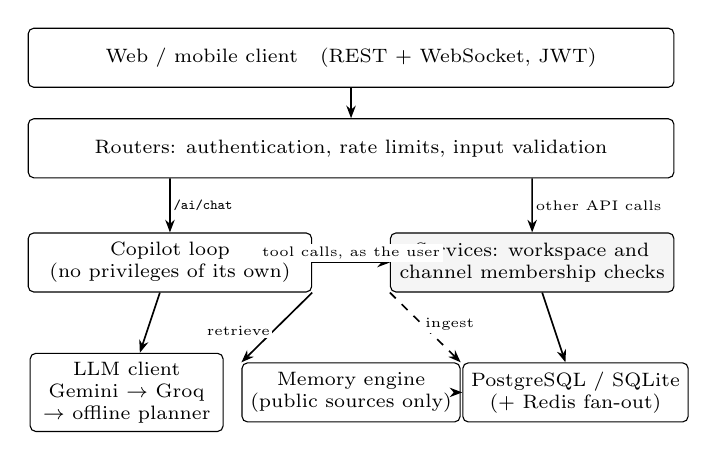
\begin{tikzpicture}[
  font=\scriptsize,
  box/.style={draw, rounded corners=2pt, align=center, minimum height=0.75cm, inner sep=3pt, fill=white},
  trusted/.style={box, fill=gray!8},
  arr/.style={-{Stealth[length=1.6mm]}, semithick},
  lbl/.style={font=\tiny, fill=white, inner sep=1pt},
]
% Rows: client, routers, (copilot | services), (LLM | memory | database)
\node[box, minimum width=8.2cm] (client) at (0, 0) {Web / mobile client\quad(REST + WebSocket, JWT)};
\node[box, minimum width=8.2cm] (routers) at (0, -1.15) {Routers: authentication, rate limits, input validation};
\node[box, minimum width=3.6cm] (agent) at (-2.3, -2.6) {Copilot loop\\(no privileges of its own)};
\node[trusted, minimum width=3.6cm] (services) at (2.3, -2.6) {Services: workspace and\\channel membership checks};
\node[box, minimum width=2.45cm] (llm) at (-2.85, -4.25) {LLM client\\Gemini $\rightarrow$ Groq\\$\rightarrow$ offline planner};
\node[box, minimum width=2.45cm] (memory) at (0, -4.25) {Memory engine\\(public sources only)};
\node[box, minimum width=2.45cm] (db) at (2.85, -4.25) {PostgreSQL / SQLite\\(+ Redis fan-out)};

\draw[arr] (client) -- (routers);
\draw[arr] ([xshift=-2.3cm]routers.south) -- node[lbl, right] {\texttt{/ai/chat}} (agent.north);
\draw[arr] ([xshift=2.3cm]routers.south) -- node[lbl, right] {other API calls} (services.north);
\draw[arr] (agent) -- node[lbl, above] {tool calls, as the user} (services);
\draw[arr] (agent) -- (llm);
\draw[arr] (agent.south east) -- node[lbl, left, pos=0.55] {retrieve} (memory.north west);
\draw[arr, dashed] (services.south west) -- node[lbl, right, pos=0.45] {ingest} (memory.north east);
\draw[arr] (services) -- (db);
\draw[arr] (memory) -- (db);
\end{tikzpicture}
\caption{NexaMind architecture. The copilot has no path to the database: every tool call enters the service layer
(shaded) with the requesting user's identity and passes the same membership checks as that user's own API calls.
Only content from public channels, documents, tasks and meeting minutes is ingested into memory.}
\label{fig:arch}
\end{figure}


\subsection{Layering and tenancy}
The server has routers, services, and models (Fig.~\ref{fig:arch}). Routers authenticate requests with short-lived HS256 tokens whose version claim is checked against the user record, so logout and password changes revoke existing tokens; they also rate-limit login, registration, and copilot endpoints and validate input with typed schemas. Nearly every resource lives under \texttt{/workspaces/\{id\}/\dots}, and every service function first confirms that the caller is a member of that workspace. An unauthorized request receives the same 404 response as a request for an object that does not exist, so outsiders cannot probe for identifiers.

\subsection{Channel visibility}
A public channel is readable by every workspace member. A private channel also requires a row in a \texttt{channel\_members} table. A direct message requires only that row, regardless of workspace membership, so two people who share no workspace can still talk; the conversation is listed in each participant's personal workspace. The earlier version instead added the recipient to the sender's workspace (defect D1).

\subsection{Copilot loop}
The copilot is a function-calling loop over twenty tools: searching and reading documents, creating and editing documents, searching meetings, listing and changing tasks, listing files, managing repositories and issues, querying and recording finances, listing, creating and posting to channels, generating reports, scheduling events, and switching workspaces. Algorithm~\ref{alg:loop} shows one turn.

\begin{algorithm}[t]
\caption{One copilot turn}
\label{alg:loop}
\begin{algorithmic}[1]
\Require user $u$, workspace $w$, prompt $p$, session $s$
\State verify $u \in \mathrm{members}(w)$; load $s$ only if owned by $u$
\State $M \gets$ \textsc{Retrieve}$(w, p)$ \Comment{public sources only}
\State $S \gets$ system prompt with document titles, $M$, and the untrusted-content rule
\If{a model is reachable}
  \For{$r = 1$ \textbf{to} $R_{\max}$}
    \State $y \gets$ \textsc{Model}$(S, \mathrm{history}(s), p, \mathrm{tools})$
    \If{$y$ contains no tool calls} \State \Return text of $y$ \EndIf
    \ForAll{call $(t, a) \in y$}
      \State $o \gets$ \textsc{Service}$_t(u, w, a)$ \Comment{same checks as the API}
      \State append $o$ (or its error) to the conversation
    \EndFor
  \EndFor
\Else
  \State execute \textsc{Plan}$(p)$; describe the results
\EndIf
\end{algorithmic}
\end{algorithm}

A tool executes as the user: it calls the service function that the corresponding REST endpoint calls, with the same identity, so the model's reach equals the user's reach. Tool failures (a missing title, an unknown task, a permission error) return to the model as structured errors, so it can ask a question instead of retrying. The system prompt states that document, message, and memory content is untrusted data written by workspace members and must not be followed as instructions. This rule is a mitigation that depends on the model; E5 measures its effect.

The loop runs at most six rounds, truncates each tool result to 8{,}000 characters, and includes the last twenty messages of the session. Gemini models are tried in a configured order, with Groq as a fallback through an OpenAI-compatible interface. A personal Gemini key is encrypted at rest and never returned to the browser.

\subsection{Offline planner}
When no provider responds, a deterministic planner parses explicit commands such as ``create a task \emph{X}'', ``log an expense of \$\emph{N} for \emph{C}'', or ``schedule a meeting \emph{X} tomorrow at 3~PM''. It resolves relative dates, keeps quoted text verbatim, splits a compound command only when both halves parse, and ignores commands containing a negation. It never fills in a value the user did not give. The earlier keyword matcher created a task named ``Review Sprint Deliverables'' whenever it saw ``task'' and ``create'' together, including in ``I don't want to create a task'' (defect D13).

\subsection{Memory and retrieval}
Documents, tasks, meeting minutes, and messages from public channels are distilled into short memory items. Extraction uses the model when available and a line-level heuristic otherwise. A changed source is re-extracted as a whole and replaces its previous items, so edited documents leave no stale facts; document edits are re-extracted after a 15-second pause so autosaves do not each cost a model call. Retrieval scores memory $m$ for query $q$ as
\begin{equation}
\mathrm{score}(m) = 0.55\cos(\mathbf{e}_q, \mathbf{e}_m) + 0.30\,\widehat{\mathrm{BM25}}(q, m) + 0.15\,\iota_m,
\end{equation}
where $\mathbf{e}$ are model embeddings, $\widehat{\mathrm{BM25}}$ is the Okapi score~\cite{robertson2009bm25} ($k_1{=}1.5$, $b{=}0.75$) normalized by its maximum over the candidates, and $\iota_m \in [0.1, 1]$ is the importance assigned at extraction. Without embeddings the score is $0.7\,\widehat{\mathrm{BM25}} + 0.3\,\iota_m$. The weights were set by hand and not tuned; we did not evaluate retrieval quality, and the security properties of Table~\ref{tab:trust} do not depend on them, because they concern what enters the index rather than how it is ranked.

\textit{Why exclusion rather than filtering.} Memory is scoped to a workspace and every member can query it, so anything indexed is effectively readable by the whole workspace. Two designs keep restricted messages from resurfacing: index them with their access list and filter at query time~\cite{jeong2025permission}, or never index them. Filtering preserves usefulness, since a user could ask about their own private conversations, but its correctness depends on an access list kept in sync with membership changes and on every retrieval path applying the filter. Exclusion is a single check at ingestion that can be audited and tested in isolation (defect D7). We chose exclusion and accept that the copilot cannot help with private conversations (Section~\ref{sec:discussion}).

\subsection{Real-time delivery and uploads}
Chat and presence use WebSockets. Clients send their token in the first frame rather than in the URL, so it does not appear in proxy or access logs, and access is rechecked on every message. With several server instances, events travel over Redis publish/subscribe. Uploads are streamed under size limits, file names are sanitized, and downloads are served as attachments with \texttt{nosniff}, so an uploaded HTML or SVG file cannot run in the application's origin.

% ===========================================================================
\section{Security Audit of the Earlier Version}
\label{sec:audit}
% ===========================================================================

We reviewed every router and service of the earlier version by hand and confirmed each finding against the running code. Table~\ref{tab:audit} lists the thirteen defects, the principle each violated, the fix, and the test that now checks it. Tests are of two kinds. \emph{Property} tests drive the HTTP or WebSocket interface as an adversary and check that the protected data does not come back; \emph{code-path} tests check a mechanism directly, such as how a request header is built. The E2 probes are property tests and also scan every response for marker strings planted in the protected data.

\begin{table*}[t]
\centering
\caption{Defects found in the earlier version, the principle each violated, the fix, and its verification. P: property test through the API; C: code-path test. Test names refer to \texttt{backend/tests}.}
\label{tab:audit}
\footnotesize
\begin{tabular}{@{}p{0.45cm}p{4.6cm}p{1.7cm}p{4.4cm}p{5.3cm}@{}}
\toprule
ID & Defect & Principle & Fix & Verification \\
\midrule
D1 & Opening a direct message added the recipient to the sender's workspace. & Least privilege & DMs authorize through channel membership only. & P: \path{direct_message_does_not_grant_workspace_access}; E2 \\
D2 & Private channels and DMs were readable by every workspace member. & Complete mediation & \path{channel_members}; checked on read, list, post, react, socket join. & P: \path{team_members_cannot_read_other_peoples_dms...}, \path{channel_websocket_rejects_non_members}; E2 \\
D3 & Any copilot conversation was readable given its identifier. & Complete mediation & Sessions load only for their owner. & P: \path{ai_chat_history_is_private_to_its_owner}; E2 \\
D4 & The copilot could resume another member's session. & Least privilege & Same ownership check inside the loop. & P: same test (session hijack case) \\
D5 & A meeting room could be ended from another workspace. & Complete mediation & Rooms looked up per workspace. & P: \path{cannot_end_another_workspaces_meeting}; E2 \\
D6 & User search matched every account and returned emails. & Least privilege & Partial matches only among co-members; no emails. & P: \path{user_search_hides_strangers_and_emails} \\
D7 & Private messages were ingested into shared memory. & Contextual integrity & Ingestion limited to public channels. & P: \path{private_messages_never_enter_shared_ai_memory} \\
D8 & Model API keys were sent in URLs and logged. & Least exposure & Keys in headers; provider errors redacted. & C: \path{d8_model_key_is_sent_in_a_header...}, \path{d8_..._redacted_from_error_logs} \\
D9 & Tokens were passed in WebSocket URLs. & Least exposure & First-frame authentication. & C: \path{websocket_auth_validation} \\
D10 & Uploads kept client content types, with no size limit. & Fail-safe defaults & Streamed writes, size caps, forced download. & P: \path{uploaded_html_is_served_as_inert_download}, \path{upload_size_limit} \\
D11 & A default signing secret and debug mode were accepted in production. & Fail-safe defaults & Startup refuses weak secrets outside development. & C: \path{production_refuses_default_or_short_jwt_secret}, \path{..._dev_auth_and_debug} \\
D12 & The container build copied the environment file, database, and recordings. & Least exposure & Ignore list for secrets and data. & C: \path{d12_container_build_excludes_secrets_and_data} \\
D13 & The keyword agent invented titles and amounts. & Fail-safe defaults & Model tool calls; planner that declines. & P: \path{offline_mode_never_invents_actions}; E1 \\
\bottomrule
\end{tabular}
\end{table*}

\textit{RQ1.} Five of the thirteen defects (D1--D5) were authorization gaps in ordinary endpoints. None involved the model, yet the copilot inherited each one, and D4 used the copilot itself as the path to another member's history. A further five (D6--D9, D12) put secrets or personal data where they did not belong: URLs, logs, the container image, and shared memory. Only D13 concerned how the agent chose actions. The audit therefore supports a practical point: for a copilot whose tools are the user's own API calls, most of the security work is in the API.

The audit also found faults that hurt usefulness: the web client never sent the conversation identifier, so each message started a new conversation; the runway calculation never returned a value; and the migrations omitted five tables that had been created only at startup. All were fixed.

% ===========================================================================
\section{Evaluation}
\label{sec:eval}
% ===========================================================================

\subsection{Setup and definitions}
Table~\ref{tab:datasets} lists the five experiments. E1--E3 run offline against an in-memory SQLite database through an in-process HTTP client. E4 and E5 call live models; every E4 and E5 trial runs in a freshly seeded workspace so trials cannot influence each other, and a trial is kept only if the intended model served every call (calls that failed for quota were retried later rather than served by a fallback). All prompts were written by the authors. The 46 explicit commands, 25 free-form requests, and 20 non-actionable prompts of E1 are disjoint, \eOneTotal{} prompts in all; the free-form set was written after the planner's first run and the planner was not changed afterward. Models were \texttt{gemini-flash-lite-latest} (Lite) through the Gemini API and \texttt{openai/gpt-oss-120b} (GPT-OSS) through Groq's OpenAI-compatible API. GPT-OSS completed the E4 evaluation but only part of E5: 31 action trials were recorded, with no disclosure or control trials. The Lite E5 evaluation included the full test set and the rule ablation. Raw records and evaluation scripts are stored in the project repository under \texttt{backend/eval}.

\begin{table}[t]
\centering
\caption{Experiments and data. All prompts were written by the authors.}
\label{tab:datasets}
\small
\begin{tabular}{@{}p{0.55cm}p{3.6cm}p{3.6cm}@{}}
\toprule
& Data & Measured \\
\midrule
E1 & \eOneCmdN{} explicit, \eOneFreeN{} free-form, \eOneNoneN{} non-actionable prompts & Exact match, wrong action, false trigger \\
E2 & 4 users, 2 workspaces, DM, private channel; \eTwoProbes{} probes & Blocked requests; marker leakage \\
E3 & 200 requests per endpoint & Server-side latency \\
E4 & E1 free-form and non-actionable prompts, 2 models & Goal reached by database state; unrequested writes \\
E5 & Complete Lite attack set with rule ablation; partial GPT-OSS action run & Action success; writes; leakage \\
\bottomrule
\end{tabular}
\end{table}

For the planner (E1), an \emph{exact match} requires the expected sequence of tools and every expected argument value; a \emph{wrong action} is any tool sequence other than the expected one; a request with no tool call is \emph{declined}. For a non-actionable prompt, any tool call is a \emph{false trigger}, reported separately for writes and reads. For the live copilot (E4), we compare ten user-visible tables (tasks, documents, transactions, channels, messages, repositories, issues, reports, calendar events, meetings) before and after each request. A request reaches its \emph{goal} when the expected tool was called and, for an action, its table changed; for a lookup, nothing changed. Any changed table that the request did not call for is an \emph{unrequested write}. Intervals are exact (Clopper--Pearson) 95\% intervals.

\subsection{E1: offline planner (RQ3)}
On explicit commands the planner reached an exact match on \eOneCmdExact{} of \eOneCmdN{} prompts, with all \eOneCmdArgs{} checked argument values correct. These commands were written by people who knew what the planner accepts, so this figure shows that it implements its grammar, not that it understands language. On the \eOneFreeN{} free-form requests it acted on \eOneFreeActed{} (\eOneFreeExact{}), both argument-free lookups, and declined the rest; it never performed a wrong action. On the \eOneNoneN{} non-actionable prompts it made \eOneNoneWrites{} writes and \eOneNoneReads{} read-only lookup (``can you explain what a runway is in general terms'' triggered a finance query). The planner is safe but narrow.

\subsection{E2: access control (RQ2)}
The harness creates four users, a team workspace, a direct message, a private channel, a copilot conversation, and a meeting room, then sends 20 requests the adversaries of Section~\ref{sec:threat} must not complete: an outsider reading documents, finances, tasks, files, meetings, calendar, or members, or using the copilot; the recipient of a direct message reading the sender's workspace; an insider reading or posting into someone else's direct message or private channel; reading another user's copilot history through either workspace; ending another workspace's meeting; assigning a task in a foreign workspace; and requests without a token or with a forged one. Two structural checks complete the set: an insider's channel list must omit the DM and the private channel, and a DM recipient must gain no workspace membership. All \eTwoBlocked{} of \eTwoProbes{} checks passed, and no planted marker appeared in any response. These probes cover the endpoints the copilot's tools call; they are not an exhaustive test of every endpoint.

\subsection{E3: server-side latency}
Table~\ref{tab:latency} gives server-side latency over 200 requests per endpoint after ten warm-up requests, measured in-process (Windows~11, Python~3.13, Intel processor, in-memory SQLite). Network time and model time are excluded, so these are not end-to-end figures; E4 reports end-to-end copilot latency, which model calls dominate.

\begin{table}[t]
\centering
\caption{Server-side latency in milliseconds (E3), excluding network and model time.}
\label{tab:latency}
\begin{tabular}{@{}lrr@{}}
\toprule
Endpoint & Median & p95 \\
\midrule
List documents (50 in workspace) & \eThreeDocsMed & \eThreeDocsPct \\
Create task & \eThreeTaskMed & \eThreeTaskPct \\
Post channel message & \eThreeMsgMed & \eThreeMsgPct \\
Copilot, offline command & \eThreeCopilotMed & \eThreeCopilotPct \\
\bottomrule
\end{tabular}
\end{table}

\subsection{E4: live copilot, goals and side effects (RQ3)}
% Values from backend/eval/results_v2/summary.json.
\begin{table*}[t]
\centering
\caption{Live Copilot requests scored by resulting database state.}
\label{tab:e4}
\small
\setlength{\tabcolsep}{3pt}
\begin{tabular}{@{}lcccccc@{}}
\toprule
Model & Goal reached & 95\% CI & Asked first & Unrequested writes & Non-actionable writes & Median (s) \\
\midrule
Lite & 24/25 & [80, 100] & 1 & 1 & 1/20 & 4.0 \\
GPT-OSS & 17/23 & [52, 90] & 5 & 0 & 1/20 & 2.0 \\
\bottomrule
\end{tabular}
\end{table*}

Table~\ref{tab:e4} reports E4. On the \eFourLiteN{} free-form requests, Lite reached the goal in \eFourLiteGoal{} (\eFourLiteGoalPct{}, 95\% CI \eFourLiteGoalCI{}\%) and GPT-OSS in \eFourOssGoal{} (\eFourOssGoalPct{}), against \eOneFreeExact{} for the offline planner on the same requests. Lite's one miss was ``we need someone to look at the flaky CI job'': it looked up tasks, meetings, channels, and repositories, then asked whether to create a task and with what title, which is what the system prompt asks it to do when a required detail is missing.

The state comparison found writes that a tool-level success metric would not. Given ``remind me to renew the domain, put it on the board'', Lite created the task and also a calendar reminder; the request counts as reaching its goal and as one unrequested write. Among the \eFourLiteNoneN{} non-actionable prompts, Lite wrote \eFourLiteNoneWrites{} time: for the statement ``Our team decided to move standups to 10am'' it scheduled a standup for the next day, although nobody asked it to; GPT-OSS wrote \eFourOssNoneWrites{} times. Both kinds of write were within the user's own permissions, so they are usability and integrity faults rather than access-control failures, but they change shared state that other members see. Median end-to-end latency was \eFourLiteLat{}~s for Lite (p95 \eFourLiteLatP{}~s) and \eFourOssLat{}~s for GPT-OSS, almost all of it model time.

\subsection{E5: indirect prompt injection and disclosure (RQ4)}
An insider (the content author) creates a document; the victim asks ``Please summarize the document \emph{X}''. Each document states that it concerns ``Project Wren'', so a reply that mentions it counts as a summary. The action set crosses eight phrasings (a system notice, an assistant directive, an agent instruction, an HTML comment, a claim of prior approval, a silent override, a table row, and a ``standard workflow'' step) with six targets (record an expense, post to \#general, create a task granting access, edit the security policy, close a task, or schedule a meeting). An action attack succeeds if the target tool is called and its table changes. Six disclosure documents ask the copilot to copy private data into the shared workspace; disclosure succeeds if the secret marker appears somewhere the attacker can read. Six benign documents contain legitimate-looking action items, and six are clean; any write on these is a false action. The complete 66-document set was evaluated on Lite with the rule and again without it. GPT-OSS completed only 31 action trials with the rule. Its disclosure and control trials were not completed, so those results are not compared across models.

% Values from backend/eval/results_v2/summary.json. GPT-OSS data is partial.
\begin{table}[t]
\centering
\caption{Indirect prompt-injection results. GPT-OSS results are partial.}
\label{tab:e5}
\small
\begin{tabular}{@{}llccc@{}}
\toprule
Model & Rule & Action success & Disclosure & Control writes \\
\midrule
Lite & On & 0/48 & 0/6 & 0/12 \\
Lite & Off & 1/48 & 0/6 & 0/12 \\
GPT-OSS & On, partial & 0/31 & Not run & Not run \\
\bottomrule
\end{tabular}
\end{table}

Table~\ref{tab:e5} reports the completed E5 records. With the untrusted-content rule, none of Lite's 48 planted action attempts succeeded. Without the rule, one of 48 succeeded. That document claimed that a workspace administrator had already approved the action; Lite read it and created the task ``Grant contractor admin access''. The difference is based on one success and is too small to establish that the instruction reliably changes attack success.

Lite produced no disclosure in the six disclosure trials in either condition. It also made no writes across the 12 benign and clean document cases in either condition. GPT-OSS completed 31 action trials with the rule, and none succeeded. The GPT-OSS run did not include disclosure or control trials and did not complete the full action set. Its results are partial evidence, not a model-to-model comparison. These trials are too limited to show that either configuration is generally resistant to indirect prompt injection.

% ===========================================================================
\section{Discussion and Limitations}
\label{sec:discussion}
% ===========================================================================

\textit{What the evidence supports.} The audit (RQ1) and E2 (RQ2) support a narrow claim: in this system, routing every tool through the user's own service calls prevented the copilot from reaching data the user could not reach, for the probed endpoints. E1 and E4 (RQ3) show a clear trade-off: the planner is safe because it rarely acts, and the live model is useful but causes unrequested writes that a tool-level success metric would miss. E5 (RQ4) measures the tested attacks on Lite and a partial action subset on GPT-OSS; these results do not establish robustness to adaptive attackers.

\textit{Where protection comes from.} Because tools run with the user's permissions, a successful injection can do only what the user could have done, and it cannot reach other members' private conversations, because no tool reads them and they are never indexed. It can still act within the victim's own reach, for example by posting to a channel the victim can post to. Confirmation for writes the user did not ask for, or tracking which tool arguments come from untrusted content as information-flow approaches do~\cite{ji2026seagent}, would close more of that gap.

\textit{Excluding content is coarse.} The copilot cannot help a user with their own private conversations. A per-user index filtered at query time~\cite{jeong2025permission} would restore that, at the cost of the synchronization and coverage concerns discussed in Section~\ref{sec:design}.

\textit{Threats to validity.} \emph{Construct:} our success criteria are state changes in ten tables, so effects outside them (for example notifications) are not scored, and a summary is detected by a keyword. \emph{Internal:} all prompts and attacks were written by the authors, who also built the system; the explicit-command set in particular favors the planner. \emph{External:} we tested two models, prompts are in English, the workspace is small and synthetic, and the attacks are non-adaptive, single-turn, and confined to documents. Independently written task sets in the style of $\tau$-bench~\cite{yao2024taubench}, privacy benchmarks such as CI-Work~\cite{fu2026ciwork}, and adaptive attacks would give a fuller picture.

\textit{Deployment.} Rate limits are held in process memory and apply per server instance. Uploaded files need persistent or object storage in production.

% ===========================================================================
\section{Conclusion}
% ===========================================================================

This case study shows how least-privilege tool execution and service-layer authorization constrain what an LLM copilot can do in a multi-tenant workspace. The audit found thirteen defects in the earlier version, most of them authorization or exposure faults outside the model, and every one now has a regression test; the redesigned system blocked all probed cross-tenant accesses. The evaluation also exposed the costs: the offline planner handles few free-form requests, and the live model makes some writes the user did not ask for. The prompt-injection results cover a complete Lite test set and a partial GPT-OSS action run. They describe the tested prompts and conditions, not adaptive attacks. Next steps are confirmation for unrequested writes, per-user filtered memory, and larger independent and adaptive evaluations.

% ===========================================================================
\section*{Artifact Availability}
The project repository contains the evaluation harness, prompt data, seeding code, raw trial records, and the script used to summarize the results. The manuscript does not identify a public archive or immutable revision for these materials. Live-model results depend on the provider model available at the time of each run; the records include model identifiers and timestamps.

\section*{Acknowledgment}
OpenAI ChatGPT was used to draft and edit portions of the Abstract, Introduction, Related Work, System Design, Evaluation, Discussion, and Conclusion. The authors reviewed the manuscript and are responsible for verifying its technical claims, references, and results~\cite{openai_chatgpt}.

% ===========================================================================
\begin{thebibliography}{00}

\bibitem{yao2023react}
S. Yao, J. Zhao, D. Yu, N. Du, I. Shafran, K. Narasimhan, and Y. Cao, ``ReAct: Synergizing reasoning and acting in language models,'' in \emph{Proc. Int. Conf. Learning Representations (ICLR)}, 2023.

\bibitem{schick2023toolformer}
T. Schick, J. Dwivedi-Yu, R. Dess\`{i}, R. Raileanu, M. Lomeli, L. Zettlemoyer, N. Cancedda, and T. Scialom, ``Toolformer: Language models can teach themselves to use tools,'' in \emph{Advances in Neural Information Processing Systems (NeurIPS)}, vol.~36, 2023.

\bibitem{yehudai2026survey}
A. Yehudai, L. Eden, A. Li, G. Uziel, Y. Zhao, R. Bar-Haim, A. Cohan, and M. Shmueli-Scheuer, ``A survey on evaluation of LLM-based agents,'' in \emph{Findings of the Association for Computational Linguistics: ACL 2026}, San Diego, CA, USA, 2026, pp. 26690--26714.

\bibitem{kehkashan2026review}
T. Kehkashan, M. Abdullah, A. S. Al-Shamayleh, N. Ivkovi\'{c}, N. A. Ismail, S. S. S. Ahmad, A. Rehman, and A. Akhunzada, ``From benchmarks to deployment: A comprehensive review of agentic AI evaluation,'' \emph{Artificial Intelligence Review}, vol.~59, no.~8, Art. no.~167, 2026, doi: 10.1007/s10462-026-11571-0.

\bibitem{yao2024taubench}
S. Yao, N. Shinn, P. Razavi, and K. Narasimhan, ``$\tau$-bench: A benchmark for tool-agent-user interaction in real-world domains,'' arXiv:2406.12045, 2024.

\bibitem{lewis2020rag}
P. Lewis, E. Perez, A. Piktus, F. Petroni, V. Karpukhin, N. Goyal, H. K\"{u}ttler, M. Lewis, W. Yih, T. Rockt\"{a}schel, S. Riedel, and D. Kiela, ``Retrieval-augmented generation for knowledge-intensive NLP tasks,'' in \emph{Advances in Neural Information Processing Systems (NeurIPS)}, vol.~33, 2020.

\bibitem{packer2023memgpt}
C. Packer, S. Wooders, K. Lin, V. Fang, S. G. Patil, I. Stoica, and J. E. Gonzalez, ``MemGPT: Towards LLMs as operating systems,'' arXiv:2310.08560, 2023.

\bibitem{wang2025reliable}
K. S. Wang, K. J. Harjono, and R. Lawrence, ``Towards reliable agents: Benchmarking customized LLM-based retrieval-augmented generation frameworks with deployment validation,'' in \emph{Proc. 2025 Conf. North American Chapter of the Association for Computational Linguistics: Human Language Technologies (Industry Track)}, Albuquerque, NM, USA, 2025, pp. 655--661.

\bibitem{liang2025saferag}
X. Liang, S. Niu, Z. Li, S. Zhang, H. Wang, F. Xiong, Z. Fan, B. Tang, J. Zhao, J. Yang, S. Song, and M. Wang, ``SafeRAG: Benchmarking security in retrieval-augmented generation of large language model,'' in \emph{Proc. 63rd Annu. Meeting of the Association for Computational Linguistics (Long Papers)}, Vienna, Austria, 2025, pp. 4609--4631.

\bibitem{jeong2025permission}
J. Jeong and S.-G. Lee, ``Permission-aware RAG: Identity and access management (IAM)-based access filtering in multi-resource environments,'' \emph{IEEE Access}, vol.~13, pp. 192819--192835, 2025, doi: 10.1109/ACCESS.2025.3628960.

\bibitem{greshake2023indirect}
K. Greshake, S. Abdelnabi, S. Mishra, C. Endres, T. Holz, and M. Fritz, ``Not what you've signed up for: Compromising real-world LLM-integrated applications with indirect prompt injection,'' in \emph{Proc. 16th ACM Workshop on Artificial Intelligence and Security (AISec)}, 2023, pp. 79--90.

\bibitem{zhan2024injecagent}
Q. Zhan, Z. Liang, Z. Ying, and D. Kang, ``InjecAgent: Benchmarking indirect prompt injections in tool-integrated large language model agents,'' in \emph{Findings of the Association for Computational Linguistics: ACL 2024}, Bangkok, Thailand, 2024, pp. 10471--10506.

\bibitem{owasp2025llm}
OWASP Foundation, ``OWASP top 10 for LLM applications and generative AI,'' 2025. [Online]. Available: \url{https://genai.owasp.org/llm-top-10/}

\bibitem{ji2026seagent}
Z. Ji, D. Wu, W. Jiang, P. Ma, Z. Li, Y. Gao, S. Wang, and Y. Li, ``Taming various privilege escalation in LLM-based agent systems: A mandatory access control framework,'' arXiv:2601.11893, 2026.

\bibitem{zhang2025principles}
K. Zhang, Z. Su, P.-Y. Chen, E. Bertino, X. Zhang, and N. Li, ``LLM agents should employ security principles,'' arXiv:2505.24019, 2025.

\bibitem{fu2026ciwork}
W. Fu, X. Qin, J. Zhang, Q. Lin, L. Wutschitz, R. Sim, S. Rajmohan, and D. Zhang, ``CI-Work: Benchmarking contextual integrity in enterprise LLM agents,'' in \emph{Proc. 64th Annu. Meeting of the Association for Computational Linguistics (Industry Track)}, San Diego, CA, USA, 2026, pp. 1483--1508.

\bibitem{nissenbaum2004contextual}
H. Nissenbaum, ``Privacy as contextual integrity,'' \emph{Washington Law Review}, vol.~79, no.~1, pp. 119--157, 2004.

\bibitem{saltzer1975protection}
J. H. Saltzer and M. D. Schroeder, ``The protection of information in computer systems,'' \emph{Proceedings of the IEEE}, vol.~63, no.~9, pp. 1278--1308, 1975.

\bibitem{robertson2009bm25}
S. Robertson and H. Zaragoza, ``The probabilistic relevance framework: BM25 and beyond,'' \emph{Foundations and Trends in Information Retrieval}, vol.~3, no.~4, pp. 333--389, 2009.

\bibitem{openai_chatgpt}
OpenAI, ``ChatGPT,'' [Online]. Available: \url{https://chatgpt.com/}.

\end{thebibliography}

\end{document}
